\section*{Условие}
Используя хвостовую рекурсию, разработать эффективную программу, позволяющую:
\begin{enumerate}
  \item Сформировать список из элементов числового списка, больших заданного
  значения;
  \item Сформировать список из элементов, стоящих на нечетных позициях исходного
  списка (нумерация от 0);
  \item Удалить заданный элемент из списка (один или все вхождения);
  \item Преобразовать список в множество (можно использовать ранее разработанные процедуры).
\end{enumerate}

Убедиться в правильности результатов.

\textbf{Для одного} из вариантов \textbf{ВОПРОСА} и 1-го задания \textbf{составить
таблицу}, отражающую конкретный порядок работы системы:

Т.к. резольвента хранится в виде стека, то состояние резольвенты требуется отображать
в столбик: (вершина – сверху). Новый шаг надо начинать с нового состояния резольвенты.  

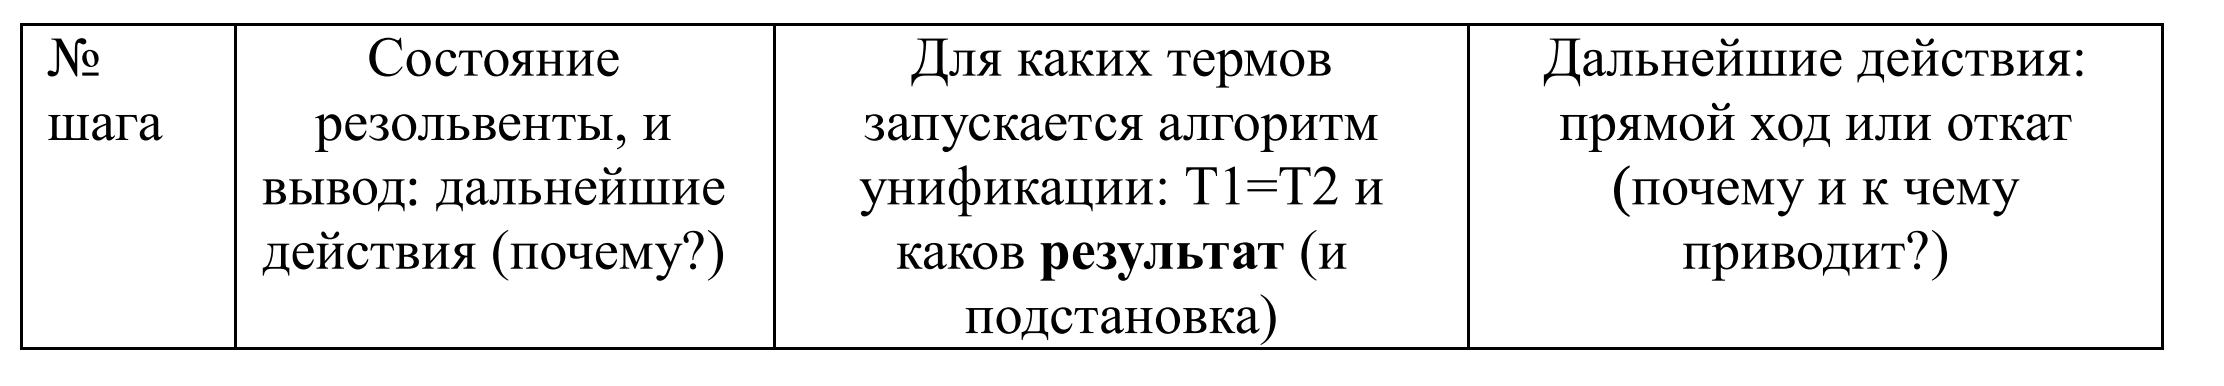
\includegraphics[scale=0.4]{./inc/img/tb_tmpl}

\clearpage

\section*{Решение}

\lstinputlisting[caption={Решение 1}, label={lst:t1}, language=Prolog]{../src/task_1.pro}

\lstinputlisting[caption={Решение 2}, label={lst:t2}, language=Prolog]{../src/task_2.pro}

\lstinputlisting[caption={Решение 3 и 4}, label={lst:t3}, language=Prolog]{../src/task_3_4.pro}

В Таблице \ref{tbl:1} представлен порядок поиска ответа на вопрос 1.

\begin{landscape}
  \setlength{\LTcapwidth}{\linewidth}
  \begin{longtable}{|c|c|c|c|c|}
      \caption[Порядок формирования результата для 1-го вопроса]{Порядок формирования результата для 1-го вопроса} \label{tbl:1}\\
  
      \hline
          Шаг & Сравниваемые термы; & Дальнейшие & Резольвента & Подстановка \\
              & результаты & действия & & \\
      \endfirsthead
  
      \multicolumn{5}{l}
      {{\tablename\ \thetable{} -- продолжение}} \\
      \hline 
          Шаг & Сравниваемые термы; & Дальнейшие & Резольвента & Подстановка \\
              & результаты & действия & & \\\hline
      \endhead
      
      \hline \multicolumn{5}{|r|}{{Продолжение на следующей странице}} \\ \hline
      \endfoot
      
      \hline \multicolumn{5}{|r|}{{Конец таблицы}} \\ \hline
      \endlastfoot
      
      \hline
            & f([2, 6, 4, 2], 3, R). & Прямой ход & 2 > 3 & H = 2\\
          1 & и f([H|T], El, [H|Res]) & & ! & T = [6, 4, 2]\\
      & & & f([6, 4, 2], 3, Res) & El = 3\\
    \hline
            & 2 > 3 & Откат & ! & H = 2\\
          2 & & & f([6, 4, 2], 3, Res) & T = [6, 4, 2]\\
      & & & & El = 3\\
    \hline
            & f([2, 6, 4, 2], 3, R). & Прямой ход & f([6, 4, 2], 3, R) & T = [6, 4, 2]\\
          3 & и f([\_|T], El, [H|Res]) & & & El = 3\\
      & & & & \\
    \hline
      & f([6, 4, 2], 3, R). & Прямой ход & 6 > 3 & H = 6\\
          4 & и f([H|T], El, [H|Res]) & & ! & T = [4, 2]\\
      & & & f([4, 2], 3, Res) & El = 3\\
    \hline
      & 6 > 3  & Прямой ход & ! & H = 6\\
          5 & & & f([4, 2], 3, Res) & T = [4, 2]\\
      & & &  & El = 3\\
    \hline
            & ! & Прямой ход & f([4, 2], 3, Res) & H = 6\\
          6 & & & & T = [4, 2]\\
      & & & & El = 3\\
    \hline
    \hline
    \dots & \dots & \dots & \dots & \dots \\
    \hline 
    0 & f([], 3, []) & Прямой ход & ! & Res = [6, 4]\\
            & и f([], \_, []) & & &\\
          \hline 
    0 & ! & Завершение & ! & Res = [6, 4]\\
            & & 1 подст. & &\\
            & & в рез-те & &\\
  \end{longtable}
\end{landscape}

\section*{Контрольные вопросы}

\subsection*{Что такое рекурсия?}

Рекурсия – это ссылка на описываемый объект при описании объекта.

\subsection*{Как организуется хвостовая рекурсия в Prolog?}

\begin{itemize}
    \item рекурсивный вызов один, расположен в конце тела правила;
    \item не должно быть возможности сделать откат до вычисления рекурсивного вызова.
\end{itemize}

\subsection*{Как организовать выход из рекурсии в Prolog?}

С помощью отсечения

\subsection*{Какое первое состояние резольвенты?}

Заданный вопрос (goal).

\subsection*{В каких пределах программы переменные уникальны?}

Именованная переменная уникальна в предложении, в котором она используется. Анонимные переменные всегда уникальны.

\subsection*{В какой момент, и каким образом системе удается получить доступ к голове списка?}

Получить голову или хвост списка можно при унификации списка с [H|T], H -- голова списка, T -– хвост списка.

\subsection*{Каково назначение и результат использования алгоритма унификации?}

Унификация – логический вывод. Результат – подстановка.

\subsection*{Как формируется новое состояние резольвенты?}

Преобразования резольвенты выполняются с помощью редукции. Редукцией цели G с помощью программы P называется замена цели G телом того правила из P, заголовок которого унифицируется с целью. Новая резольвента образуется в два этапа:
\begin{itemize}
    \item в текущей резольвенте выбирается одна из подцелей и для неё выполняется редукция;
    \item к полученной конъюнкции целей применяется подстановка, полученная как наибольший общий унификатор цели и заголовка сопоставленного с ней правила.
\end{itemize}

\subsection*{Как применяется подстановка, полученная с помощью алгоритма унификации?}

Подстановка применяется к целям в резольвенте путем замены текущей переменной на соответствующий терм.

\subsection*{В каких случаях запускается механизм отката?}

Механизм отката запустится в случае неудачи алгоритма унификации.

\subsection*{Когда останавливается работа системы?}

Работа системы останавливается, когда найдены все возможные ответы на вопрос.

\subsection*{Как это определяется на формальном уровне?}

Когда в резольвенте находится исходный вопрос, для которого пройдена вся БЗ.